\documentclass[10pt,lot,lof]{puthesis_undergraduate}
\usepackage{amsfonts}
\usepackage{amssymb}
\usepackage{amsmath}
\usepackage{amsthm}
\usepackage{latexsym}
\usepackage{color}
\usepackage{graphicx}
\DeclareGraphicsExtensions{.pdf,.png,.jpg}
\usepackage{float}
\usepackage{setspace}
\usepackage[round, longnamesfirst]{natbib} % for nice bibliography

% References package
\usepackage{hyperref}
\def\sectionautorefname{Section}
\def\chapterautorefname{Chapter}

% Import and initialize code display packages
\usepackage{listings}
\usepackage{color}
\definecolor{dkgreen}{rgb}{0,0.6,0}
\definecolor{gray}{rgb}{0.5,0.5,0.5}
\definecolor{mauve}{rgb}{0.58,0,0.82}
\lstset{frame=tb,
  language=Java,
  aboveskip=3mm,
  belowskip=3mm,
  showstringspaces=false,
  columns=flexible,
  basicstyle={\small\ttfamily\singlespacing},
  numbers=none,
  numberstyle=\tiny\color{gray},
  keywordstyle=\color{mauve},
  commentstyle=\color{dkgreen},
  stringstyle=\color{blue},
  breaklines=true,
  breakatwhitespace=true
  tabsize=2
}

%%%%%% ENVIRONMENTS %%%%%%
%\swapnumbers
%\newtheorem{theorem}{Theorem}
%\newtheorem{proposition}[theorem]{Proposition}
%\newtheorem{lemma}[theorem]{Lemma}
%\newtheorem{definition}[theorem]{Definition}
%\newtheorem{corollary}[theorem]{Corollary}
%\newtheorem{remark}[theorem]{Remark}
%\newtheorem{conjecture}[theorem]{Conjecture}
%\newtheorem{notation}[theorem]{Notation}
%\newtheorem{example}[theorem]{Example}
%\newtheorem{exercise}{Exercise}
%\newtheorem*{notes}{Notes}

% For PUthesis.cls use the following definitions:
\newtheorem{theorem}{Theorem}[section]
\newtheorem{lemma}[theorem]{Lemma}
\newtheorem{corollary}[theorem]{Corollary}
\newtheorem{proposition}[theorem]{Proposition}
\newtheorem{definition}[theorem]{Definition}
\newtheorem{claim}{Claim}
\newtheorem{conjecture}[theorem]{Conjecture}
\newtheorem{observation}[theorem]{Observation}
\newtheorem{problem}[theorem]{Problem}



%%%%%% NEW COMMANDS/OPERATORS %%%%%%
\DeclareMathOperator{\esup}{\text{ess\;sup}}
\providecommand{\abs}[1]{\lvert#1\rvert} % absolute value function
\renewcommand{\P}{\mathbb{P}}  % probability measure
\renewcommand{\O}{\mathcal{O}} % order notation
\newcommand{\PP}{\P^\star} % pricing probability measure
\newcommand{\E}{\mathbb{E}}  % expectation
\newcommand{\Var}{\mathrm{Var}}
\newcommand{\EE}{\E^\star}   % expectation under the pricing measure
\newcommand{\V}{\text{Var}} % variance
\newcommand{\F}{\mathcal{F}} % filtration
\newcommand{\G}{\mathcal{G}} % filtration
\renewcommand{\H}{\mathcal{H}} % filtration
\newcommand{\Fb}{\mathbb{F}} % filtration
\newcommand{\N}{\mathbb{N}}  % integers
\newcommand{\R}{\mathbb{R}}  % real numbers
%\renewcommand{\C}{\mathbb{C}}  % complex numbers
\newcommand{\argmin}{\mathop{\mathrm{arg\,min}}} % arg min operator
\newcommand{\cpb}{c^{\mbox{\scriptsize pb}}} % protection buyer payment
\newcommand{\cps}{c^{\mbox{\scriptsize ps}}} % protection seller payment
\newcommand{\cds}{c^{\mbox{\scriptsize ds}}} % CDS spread

\newcommand{\T}{\mathcal{T}} % tenor
\renewcommand{\vec}[1]{\mbox{\boldmath $#1$}} % boldface 1 for the indicator function
\newcommand{\ind}{\vec{1}}                    % boldface 1 for the indicator function
\newcommand{\Ws}{W^\star_t}
\newcommand{\tWs}{\widetilde{W}^\star_t}
\newcommand{\tWz}{\widetilde{W}^0_t}
\newcommand{\tW}{\widetilde{W}}

%%%%%% Shortcut expressions %%%%%%
\newcommand{\pb}{protection buyer}
\newcommand{\ps}{protection seller}
\newcommand{\BibTeX}{{\sc Bib}\TeX}

%%%%%% Greeks %%%%%%
\newcommand{\eps}{\varepsilon}
\newcommand{\de}{\delta}
\newcommand{\fee}{\varphi}
\newcommand{\half}{\frac{1}{2}}

%%%%%% PDEs %%%%%%%
\newcommand{\pa}{\partial}
\renewcommand{\L}{\mathcal{L}}
\newcommand{\M}{\mathcal{M}}
\newcommand{\A}{\mathcal{A}}
\newcommand{\wA}{\widetilde{\A}}
\newcommand{\wlop}{\widetilde{\L}}
\newcommand{\wmop}{\widetilde{\M}}
\newcommand{\lbs}{\L_{BS}}
\newcommand{\lbss}{\L_{BS^\star}}
\newcommand{\lzero}{\L_{0}}
\newcommand{\lone}{\L_{1}}
\newcommand{\ltwo}{\L_{2}}
\newcommand{\wled}{\widetilde{\L}^{\eps,\de}}
\newcommand{\wlone}{\widetilde{\L}_1}
\newcommand{\wltwo}{\widetilde{\L}_2}
\newcommand{\cltwo}{\langle \L_2 \rangle}
\newcommand{\cwltwo}{\left\langle \wltwo \right\rangle}
\newcommand{\mone}{\M_{1}}
\newcommand{\mtwo}{\M_{2}}
\newcommand{\mthree}{\M_{3}}
\newcommand{\wmone}{\widetilde{\M}_1}
\newcommand{\fc}{\langle f \rangle}  % <f>

\newcommand{\bes}{\begin{equation*}}

%%%%%% OLD ONES %%%%%%
%\newcommand{\sigbar}{\overline{\sigma}}
%\newcommand{\sigstar}{\sigma_\star}
%\newcommand{\CBS}{C_{BS}}
%\newcommand{\CBSs}{C_{BS^\star}}
%\newcommand{\BS}{Black-Scholes }
%\newcommand{\vol}{volatility}
%\newcommand{\SV}{stochastic volatility }
%\newcommand{\PP}{{\mathord{I\kern -.33em P}}}
%\newcommand{\EE}{{\mathord{I\kern -.33em E}}}
%\newcommand{\RR}{{\mathord{I\kern -.33em R}}}
%\newcommand{\1}{{\mathord{1\kern -.26em \text{I}}}}
%\newcommand{\calp}{{\PP}}
%\newcommand{\EEE}{{\EE^{\star}}}
%\newcommand{\PPP}{{\PP^{\star}}}
%\newcommand{\ssb}{\overline{\sigma^2}}


%Do not un-comment the next two lines
%Included for Gather Purpose only in WinEdt (ignore for other editors):
%input "./Bibliography/refs.bib"

\title{Chatty Stochastic Multi-Armed Bandits}
\submitted{June 2014}  %graduation date
\author{Akshay Kumar}
\advisor{S\'{e}bastien Bubeck} %
\dedication{To Mom, Dad, Neha and Isabella}

\abstract{
This thesis uses a variant of the classic stochastic multi-armed bandit framework to improve the user experience in an anonymous chat application online by selecting good conversation starters. While the traditional algorithm would converge on the `optimal' conversation starter and use it for every conversation, this novel version of the algorithm attempts to provide new conversation starters for each user while still attempting to maximize the conversation quality. This thesis examines the empirical behavior of such an algorithm in a web application deployed at Princeton University.

}

\acknowledgements{
First and foremost, I would like to thank my parents and sister for years of love and support as I conclude my undergraduate education. I am the person that I am today because of them, and I am very proud to call them my family.

I am also grateful to Professor Bubeck for his guidance over the course of my senior year. His flexibility made this relatively un-orthodox ORFE thesis extremely enjoyable, and allowed me to spend my senior year getting excited about building something new. I am also grateful to my close friend Damjan Kora\`{c} '13 for giving excellent feedback on the first draft.

This thesis also wouldn't have been possible without the help of Daniel Kang '14, with whom I collaborated on the auxiliary, non-bandit related code in this thesis. His experience in web design and front-end development was indispensable in getting Tigers Anonymous up and running in such a short time, and his friendship made the collaboration that much more enjoyable.

Finally, I'd like to thank Isabella Chen '15 for being such a great companion over the course of this year.

FIXME ADD MORE

}

\let\savedbegincmd\begincmd
\let\begincmd\relax
\begin{document}
\savedbegincmd

\chapter{Introduction}
\label{ch:Introduction} 
At most college campuses, as students become more settled within their college community, it becomes increasingly harder to branch out and meet people outside their immediate social graph. It was in response to such a problem that Tigers Anonymous (TA) was created. By providing a way to anonymously be matched with, chat with, and potentially meet fellow classmates, TA allows students to make new connections and shake up their social network while also providing a great way to develop and test a new, weakly context-dependent variant of the classic UCB1 multi-armed bandit algorithm (the UCB1-AKSB algorithm, described fully in \autoref{ch:Methods}), which is the main focus on this thesis.

\section{What is Tigers Anonymous?}

Tigers Anonymous (TA) is the title of a chat application that allows any Princeton student to be matched with another Princeton student. After being matched, the students will be taken to an anonymous chatroom where they are given a conversation starter and have the opportunity to have a conversation. Once both participants have exchanged a pre-determined number of messages, a drop-down menu appears containing two choices (see \autoref{fig:DropDownMenu} below). If both users click "Yes", the application will authenticate both users via Facebook and reveal each users' identities to the other to facilitate communication outside of TA. For more information on how TA is implemented, see \autoref{app:TABackendImplementation} and \autoref{app:TAFrontendImplementation}.

\begin{figure}[h]
\centering
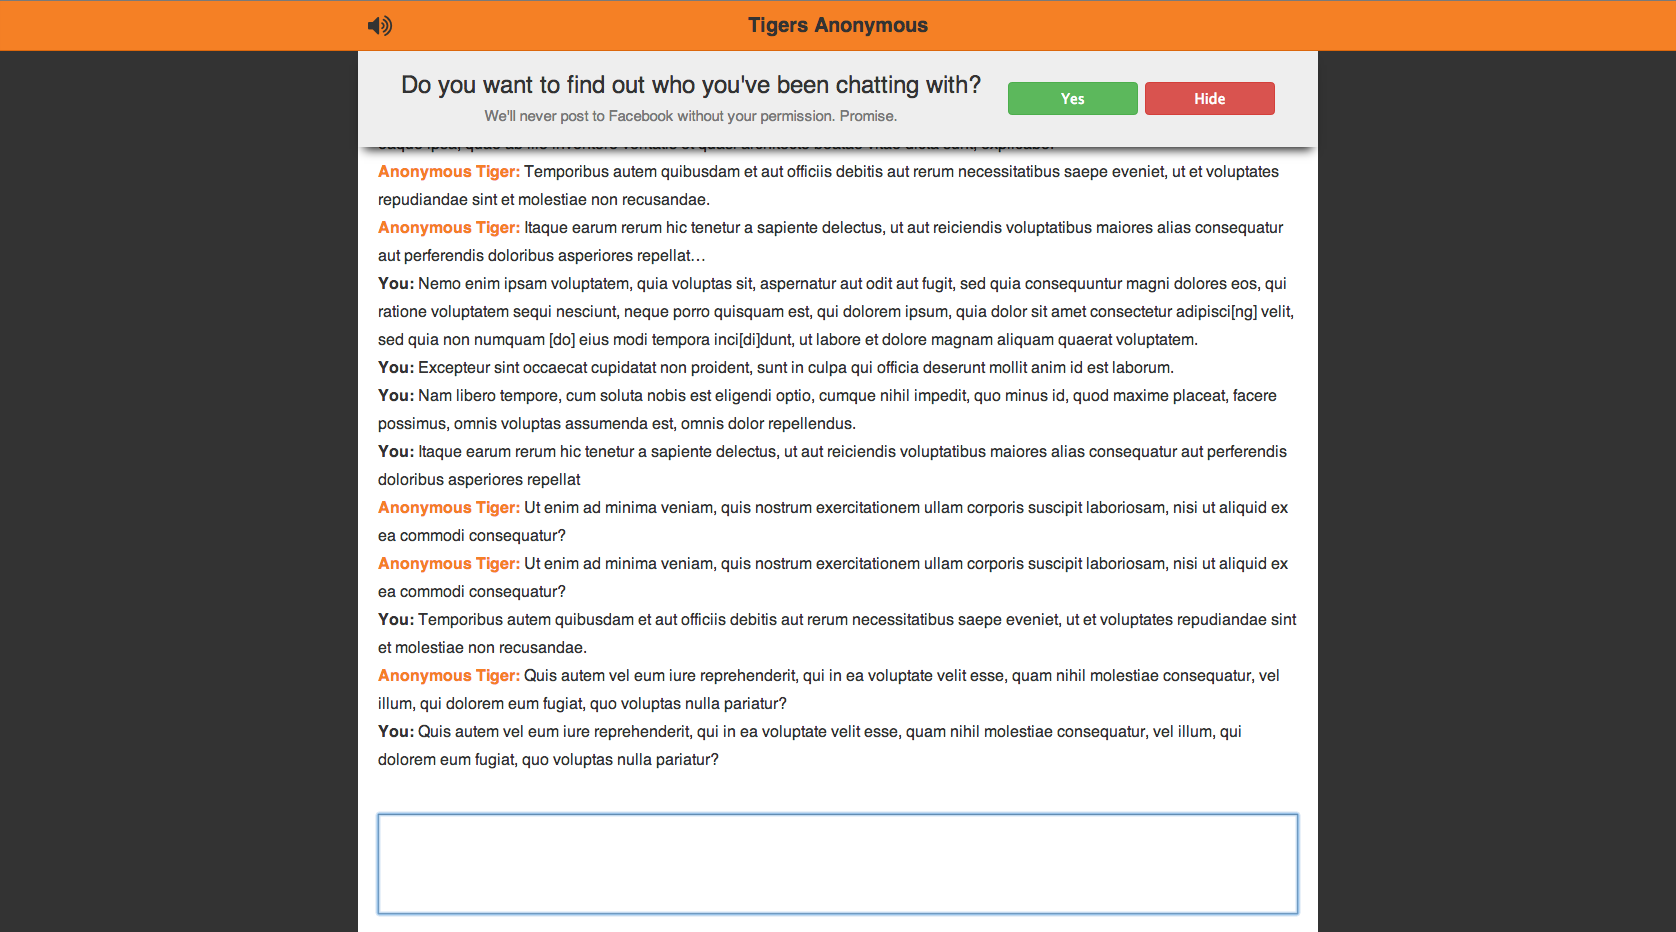
\includegraphics[trim= 120mm 0mm 120mm 0mm, clip, scale=0.36]{./Figures/FullChatDropDown}
\caption{TA Drop-Down Menu}
\label{fig:DropDownMenu}
\end{figure}

\section{Why Multi-Armed Bandits?}
\label{sec:WhyMultiArmedBandits}
A significant part of the functionality of TA is providing a conversation starter to reduce the awkwardness of the initial interaction with an anonymous stranger online. A naive approach would simply choose conversation starters at random, but this approach would be less than optimal for two reasons. First, students might respond better to some conversation starters than others, so TA should be able to hone in on the best conversation starters and display them in order to facilitate higher quality conversations. Second, users could potentially see the same conversation starter more than once in a short period of time, which would defeat the purpose of having novel conversation starters.

This is where the multi-armed bandit problem comes in. By modeling conversation starters as "arms" in a classical multi-armed bandit problem and a "success" as a "high-quality" conversation, it should be possible to solve both of the above problems. For more information on the multi-armed bandit problem and the motivation for the UCB1-AKSB algorithm described in \autoref{ch:Methods}, see \autoref{ch:LiteratureReview}.


\chapter{Background Research}
\label{ch:LiteratureReview}
In its most general form, the multi-armed bandit problem is a sequential decision-making problem where the decision-maker must explore new possibilities while trying to exploit existing knowledge to maximize the received payout. Using the notation in \cite{bubeck12}, there are are $K \geq{2}$ arms and sequences $X_{i, 1}, X_{i, 2}, ... $ for each arm $i = 1, ..., K$. At each time step, $t = 1, 2, ...$, the decision-maker picks $I_t \in \{1, ..., K\}$ and receives a payout $X_{I_t, t}$.

The common way of benchmarking the performance of a decision-making algorithm in this context is to take the distance between the expected payout of the algorithm and the optimal payout by play $n$. In the literature, optimality can be defined at two levels of granularity: at the play-by-play level or at the arm-level. Using the first notion of optimality yields the expected regret, which is defined in \autoref{eq:ExpectedRegret}.

\begin{equation}
\label{eq:ExpectedRegret}
\mathbb{E}R_n = \mathbb{E}\left[ \max_{i=1, ..., K}{\sum_{t=1}^{n}{X_{i, t}}} - \sum_{t=1}^{n}{X_{I_t, t}}\right]
\end{equation}

A slightly weaker notion of regret comes from the second, more broad definition of optimality: picking the arm with the optimal expected payout. Using this notion of optimality yields the pseudo-regret, which is defined in \autoref{eq:PseudoRegret}.

\begin{equation}
\label{eq:PseudoRegret}
\overline{R}_n = \max_{i=1, ..., K}\mathbb{E}\left[\sum_{t=1}^{n}{X_{i, t}} - \sum_{t=1}^{n}{X_{I_t, t}}\right]
\end{equation}

It is important to notice here that in \autoref{eq:ExpectedRegret}, the algorithm is competing with the best possible random draw at every time-step, whereas in \autoref{eq:PseudoRegret}, the algorithm is only competing with the arm with the highest expected value. This is the intuition for why $\overline{R}_n \leq{\mathbb{E}R_n}$.

Now that the general form of the multi-armed bandit problem has been introduced, there are three main sub-problems outlined by \cite{bubeck12} with further assumptions about the reward distributions. In the stochastic version, the sequences of plays $X_{i, 1}, X_{i, 2}, ... $ are I.I.D samples drawn from distributions $\nu_i \in [0, 1]$ for each arm $i = 1, ..., K$. In the adversarial version, at each time step $t$ an adversary selects a gain vector $g_t = (g_{1, t}, ..., g_{K, t}) \in [0, 1]^{K}$ such that $X_{i, t} = g_{i, t}$. In the Markovian version, the reward processes are neither i.i.d (as in the stochastic version) or chosen by an adversary (as in the adversarial version). Instead, each arm represents a Markov process with a state space $S$. Each time an arm $i$ is chosen in state $s \in{S}$, a reward is drawn from a probability distribution $\nu_{i, s}$ and the state of the Markov process for arm $i$ changes to $s' \in {S}$ based on a transition probability matrix $M_i$.

Armed with these three formulations of the multi-armed bandit problem, we can turn to the problem at hand: choosing conversation starters for a pair of TA users. Under the simplifying assumption that Princeton students react similarly to different conversation starters, at first glance it makes sense to use the stochastic formulation of the multi-armed bandit problem since the reward distribution could reasonably be assumed to be I.I.D. Additionally, the UCB1 algorithm in is elegant, computationally easy to implement, and has a logarithmic upper-bound on cumulative pseudo-regret when applied to a stochastic multi-armed bandit problem \citep{auer02}.

Although modeling the selection of conversation starters as a stochastic multi-armed bandit problem (and subsequently using the UCB1 algorithm) solves the first problem outlined in \autoref{sec:WhyMultiArmedBandits} (i.e. picking the conversation starter that students would respond best to), it would actually exacerbate the second problem (i.e. seeing the same conversation starter repeatedly). Since the stochastic multi-armed bandit version of the problem assumes the reward distributions are I.I.D, it will simply hone in on the distribution with the highest expected value, and in the long term, will just pick the optimal arm at every play. In the context of TA, this would result in a single conversation starter always being displayed in the long term. This, in turn, would defeat the purpose of having a variety of conversation starters in the first place.

Since the arms chosen need to depend on the context (i.e. which users are chatting), a logical first choice would be to turn to a contextual bandit algorithm formulation. One example of such a personalized recommendation algorithm can be found in \cite{chu10}. \cite{chu10} observe the current user and a set of arms along with a feature vector for each user/arm pair. This vector summarizes information of both the user and arm, and can be thought of as the context. However, such a model would rapidly get out of hand for TA for a variety of reasons. First, there isn't just one user, but rather a pair of users, so one would have to maintain an extremely sparse database of all feature vectors for all arms, for all possible pairs of users. With a reasonable user-base of 1000 users and 200 conversation starters, this would result in 200,000,000 (e.g. $200 * 1000 * 1000$) feature vectors, many of which would be empty because the user-pair had not yet been observed. Second, the actual algorithm proposed in \cite{chu10} requires matrix multiplication and inversion to calculate the UCB value for each contextual bandit, which makes it computationally costly and infeasible for a web application handling multiple concurrent requests on a single server. Finally, having such a high level of context-dependency is unnecessary given the assumption that Princeton students' responses to a given conversation starter will be I.I.D.

This raises an important question: how do we take advantage of the simplifying assumption that Princeton students will respond similarly to any given conversation starter (i.e. the rewards are I.I.D) while still enforcing the invariant that a user doesn't see the same conversation starters repeatedly? This was the motivation to create a UCB algorithm somewhere between the context-free UCB1 and the context-dependent LinUCB. This new algorithm (which I have named UCB1-AKSB) is weakly context dependent, in that it applies the context-free UCB1 algorithm but dynamically filters the arms over which the algorithm to only include arms that neither user has already seen. This intuitive explanation is formalized in \autoref{ch:Methods} below.


\chapter{Methods}
\label{ch:Methods}
\section{UCB1-AKSB Algorithm}

The multi-armed bandit algorithm used by Tigers Anonymous is a novel variant of the well-known UCB1 algorithm \citep{auer02}. The new algorithm is outlined below:

Before explaining the algorithm, it will be useful to introduce notation. Let the users be represented as the set $U$ and the bandit arms as the set $X$. Let the set of arms that have already been played for user $u\in{U}$ be represented by the set $X^u \subset{X}$. The goal of the UCB1-AKSB algorithm is to pick some arm $x\in{X}$ given the pair of users $u,v \in{U}$. In this specific application, the goal is to pick the optimal conversation starter $x\in{X}$.

The UCB1-AKSB algorithm proceeds as follows: For each pair of users $u,v\in{U}$, we pick the conversation starter $x$ such that

\begin{equation}
\label{eq:UCBMain}
x = \underset{x \in{\{X^u \cup X^v\}}^{\mathsf{c}}}{\arg\max{}} f(x)
\end{equation}
where

\begin{equation}
\label{eq:UCBMetric}
   f(x) = \left\{
     \begin{array}{lr}
       \bar{x}+ \sqrt{\frac{2\ln{n}}{n_x}} & : n_x > 0\\
       \infty & : n_x = 0
     \end{array}
   \right.
\end{equation}

In \autoref{eq:UCBMetric}, $n_x$ is the number of times that conversation starter $x$ has been played and $n$ is the total number of conversation starters that have been shown. Note that ties are broken arbitrarily. Additionally, in the event that $\{X^u \cup X^v\} \in \emptyset$, the algorithm simply selects a random arm.

\section{Tigers Anonymous Data Collection Methods}

The complete data-collection method used for this thesis is outlined below: 

\begin{enumerate}
\item Two users visit www.tigersanonymous.com/chat from a Princeton IP address.
\item The users are directed to the chat server and are matched on a first-come, first-served basis.
\item A conversation starter is selected based on the UCB1-AKSB algorithm described above.
\item After either of the users disconnects, a 10-tuple representing the chat session is logged in a database (see Data Format section below for more details).
\end{enumerate}

\section{Tigers Anonymous Data Format}

The data that will be collected can be represented by the vector of 10-tuples of the form: $$(x_i, y_i, t0_i, t1_i, q_i, b_i, c1_i, c2_i, m1_i, m2_i)$$ where $x_i$ and $y_i$ represent the pseudonymous user ids of the two participants in the chat, $t0_i$ and $t1_i$ represent the start and end times of the conversation, $q_i$ represents the conversation starter, $b_i \in {(0, 1)}$ represents whether the drop-down menu was displayed (i.e. both chat participants exchanged more than a predefined number of messages), $c1_i, c2_i \in{(0, 1)}$ represent whether users $x_i$ and $y_i$ opted to de-anonymize the conversation respectively and $m1_i, m2_i \in{(0,1)}$ represent the number of messages that user $x_i$ and $y_i$ sent respectively. The subscript $i$ is unique for each conversation. 

A sample of this data is shown below: 

\begin{lstlisting}[language=java]
[{ "userID1" : "9a675a6f581fd1dfa0b982826e75b4f5", "userID2" : "a8262bb13e641e2bf5dcb3985b2061be", "question" : "Do you believe in love at first sight?", "startTime" : 1390873110621, "endTime" : 1390873162944, "buttonDisplayed" : false, "user1Clicked" : false, "user2Clicked" : false, "user1MessagesSent" : 1, "user2MessagesSent" : 0, "_id" : "52e70a4ac43b6d020079e52d", "__v" : 0 },
{ "userID1" : "a8262bb13e641e2bf5dcb3985b2061be", "userID2" : "9a675a6f581fd1dfa0b982826e75b4f5", "question" : "Do you believe in soul mates?", "startTime" : 1390873219878, "endTime" : 1390873263469, "buttonDisplayed" : false, "user1Clicked" : false, "user2Clicked" : false, "user1MessagesSent" : 1, "user2MessagesSent" : 2, "_id" : "52e70aafc43b6d020079e52e", "__v" : 0 },
{ "userID1" : "27ac4f2d7e40b5249c2edcba19e21fb8", "userID2" : "370f85e443ad3ee24a879b1ce5a2b54b", "question" : "What is one thing you miss about being a kid?", "startTime" : 1390876198530, "endTime" : 1390876307059, "buttonDisplayed" : false, "user1Clicked" : false, "user2Clicked" : false, "user1MessagesSent" : 1, "user2MessagesSent" : 0, "_id" : "52e71693c43b6d020079e52f", "__v" : 0 },
{ "userID1" : "370f85e443ad3ee24a879b1ce5a2b54b", "userID2" : "6e0fe76fca80cf2920bd5fc7717cf6dd", "question" : "What's one thing that you learned this week?", "startTime" : 1390881063228, "endTime" : 1390882681992, "buttonDisplayed" : true, "user1Clicked" : true, "user2Clicked" : true, "user1MessagesSent" : 33, "user2MessagesSent" : 37, "_id" : "52e72f79c43b6d020079e531", "__v" : 0 },
...]
\end{lstlisting}

\section{Tigers Anonymous UCB1-AKSB Implementation}

This is the code on the Tigers Anonymous chat server that implements the UCB1-AKSB algorithm.

\lstinputlisting{./Code/ucb.js}


\chapter{Results}
\label{ch:DataAnalysis}
\section{Regret Analysis}
\label{sec:RegretAnalysis}

Recall from \autoref{ch:LiteratureReview} that the cumulative regret of the UCB1 algorithm is proportional to log($n$), where $n$ is the number of plays. Thus, we should expect the UCB1-AKSB algorithm to result in a cumulative pseudo-regret that is approximately logarithmic in the number of plays. This empirical pseudo-regret, $\hat{R}_n$, was calculated using \autoref{eq:RegretComputation} below under the assumptions that the long-term average de-anonymization proportion was optimal.

\begin{equation}
\label{eq:RegretComputation}
\hat{R}_n = \mu^{*}n - \sum_{t=1}^{n}{X_{I_t, t}}
\end{equation}

In \autoref{eq:RegretComputation}, $\mu^{*}n$ is the expected optimal number of de-anonymizations by play $n$ (i.e. $\max_{i=1,...,K}{\mathbb{E}\left[\sum_{t=1}^{n}{X_{i, t}}\right]}$ from \autoref{eq:PseudoRegret}). The plot of $\hat{R}_n$ as a function of $n$ for the UCB1-AKSB algorithm is shown below in \autoref{fig:TADe-AnonymizationRegret}.

\begin{figure}[H]
\centering
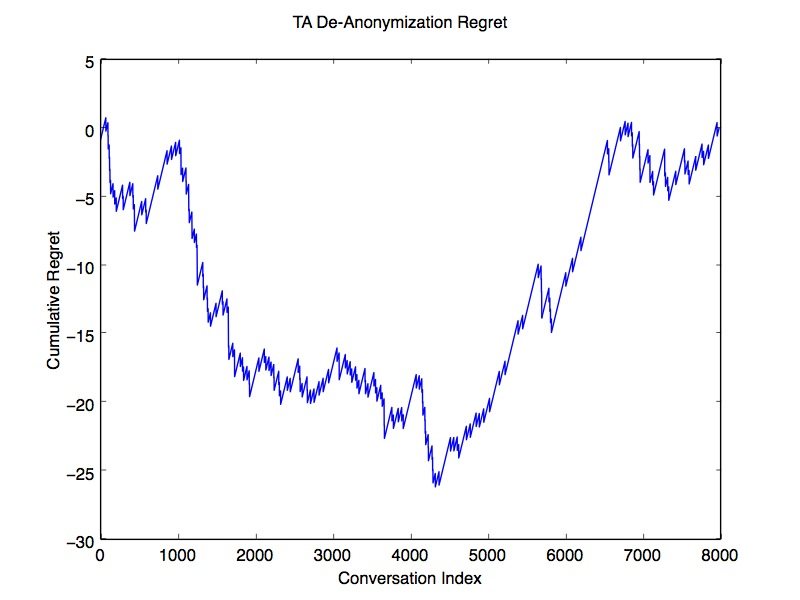
\includegraphics[trim= 0mm 0mm 0mm 0mm, clip, scale=0.5]{./Figures/TADe-AnonymizationRegret.jpg}
\caption{TA De-Anonymization Regret Analysis}
\label{fig:TADe-AnonymizationRegret}
\end{figure}

The regret looks approximately logarithmic for the second half of the dataset, but the first half of the data gives a steadily negative cumulative regret. This is due to the fact that the I.I.D assumption of conversation de-anonymization is most-likely false. Instead, there were probably different regimes in which people perceived Facebook de-anonymization differently. This is most analogous to the Markovian bandits in \cite{bubeck12}, where each conversation starter (i.e. bandit arm) is associated with a Markov process with a discrete set of distributions.

Because of the clear split in the data, it seems like there were two discrete distributions from which de-anonymizations were drawn. The first distribution occurred in the initial stages of TA's launch, where users were more likely to de-anonymize a conversation simply because of the novelty of doing so. This is supported by looking at the initial cumulative Facebook de-anonymization statistics (see \autoref{fig:TADe-AnonymizationCumulative}), where the Facebook connect rate was almost double the long-term average. The second distribution most likely occurred as users became more used to the idea of anonymity (and probably began to enjoy it), thus resulting in a lower conversation de-anonymization rate. The existence of multiple regimes explains the two parts of the regret data in \autoref{fig:TADe-AnonymizationRegret}.

\begin{figure}[H]
\centering
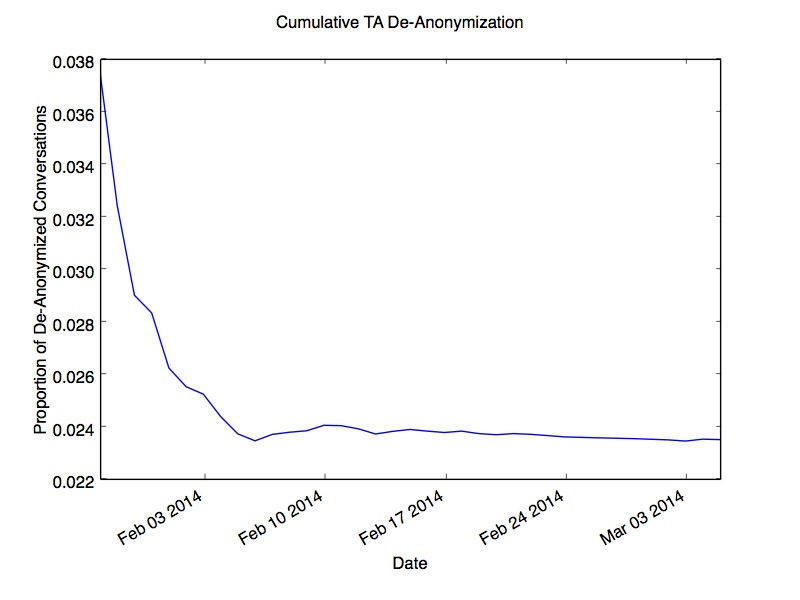
\includegraphics[trim= 0mm 0mm 0mm 0mm, clip, scale=0.5]{./Figures/CumulativeTADe-Anonymization.jpg}
\caption{TA Cumulative Conversation De-Anonymization Rate}
\label{fig:TADe-AnonymizationCumulative}
\end{figure}

\section{UCB1-AKSB Effectiveness}

Since conversation de-anonymization was the metric that UCB1-AKSB used to judge each bandit arm, the obvious way to measure the performance of the UCB1-AKSB algorithm is the proportion of conversations which were de-anonymized. Judging from not only the cumulative de-anonymization proportion (\autoref{fig:TADe-AnonymizationCumulative}), but also the daily de-anonymization proportion (\autoref{fig:TADe-AnonymizationDaily}), it seems that the algorithm had little impact on whether or not people opted to de-anonymize the conversation. If anything, it looks like the algorithm had an adverse impact on conversation de-anonymization.

However, this may have been due to the fact that the user's decision to de-anonymize the conversation was based on factors other than the conversation starter. It is easy to imagine a case in which the conversation was extremely revealing and thus users were hesitant to reveal their identities for fear of being connected to the conversation. In such cases, the conversation starter may have been excellent (and would have led to de-anonymization in some cases), but in other cases, the tendencies of the specific users would prevent them from de-anonymizing after the conversation had progressed past a certain level. In other words, the process of conversation de-anonymization might have been more user-specific (i.e. context dependent) than the UCB1-AKSB algorithm assumed, which could have resulted in a downward drag on de-anonymization rates even as the conversation starter quality improved.

Another possible explanation for falling de-anonymization rates is the increasing fascination with anonymity as mentioned in the previous section: over time, TA's perception changed from a site to make new connections to a site to have anonymous conversations, with user behavior adjusting accordingly. This is also consistent with the multiple regimes that can be seen in the cumulative psuedo-regret data in the previous section.

Finally, even if the process of conversation de-anonymization was sufficiently user-independent for the UCB1-AKSB algorithm to work properly, the metric itself is not granular to accurately measure incremental improvements. For example, let's say the conversation de-anonymization would only occur if the conversation `quality' metric was above some threshold $d$. Even if the UCB1-AKSB algorithm boosted the quality of otherwise low-quality conversation by providing some common ground, such a quality boost would not be visible unless the incremental improvement was enough to make such conversations pass the threshold $d$. Basically, it is entirely possible that the UCB1-AKSB algorithm could improve conversation quality but this increased likelihood would not be visible because of the censored data observed. This censored-data hypothesis would also explain some of the erratic behavior of the daily de-anonymization rate seen in \autoref{fig:TADe-AnonymizationDaily}.

\begin{figure}[H]
\centering
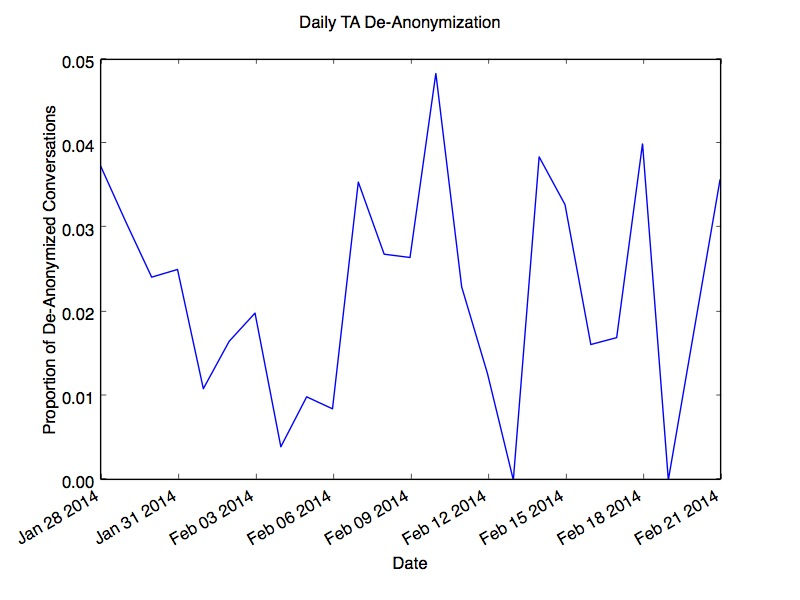
\includegraphics[trim= 0mm 0mm 0mm 0mm, clip, scale=0.5]{./Figures/DailyTADe-Anonymization.jpg}
\caption{TA Daily Conversation De-Anonymization Rate}
\label{fig:TADe-AnonymizationDaily}
\end{figure}

Given that conversation de-anonymization might have been affected by other exogenous variables and was not granular enough to measure incremental improvements in conversation quality, it makes sense to turn to other conversation quality metrics to judge the performance of UCB1-AKSB. These other metrics (participation rates and average conversation rates) are less likely to be influenced by the social pressure for or against de-anonymization, as well as having a more finely differentiated set of values than the binary variable of conversation de-anonymization. The plots of both these metrics are shown below in \autoref{fig:TAParticipationCumulative} and \autoref{fig:TAMessagesExchangedCumulative}.

\begin{figure}[H]
\centering
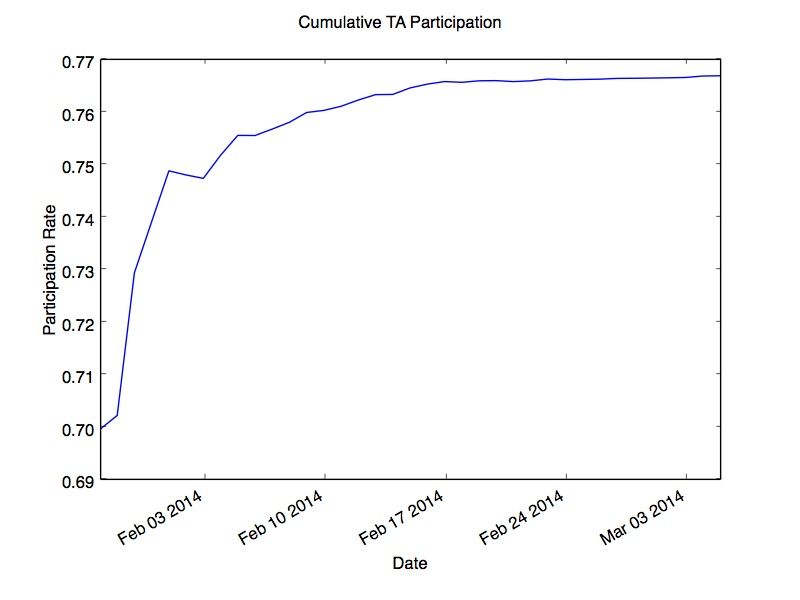
\includegraphics[trim= 0mm 0mm 0mm 0mm, clip, scale=0.5]{./Figures/CumulativeTAParticipation.jpg}
\caption{TA Cumulative Participation Rate}
\label{fig:TAParticipationCumulative}
\end{figure}

\begin{figure}[H]
\centering
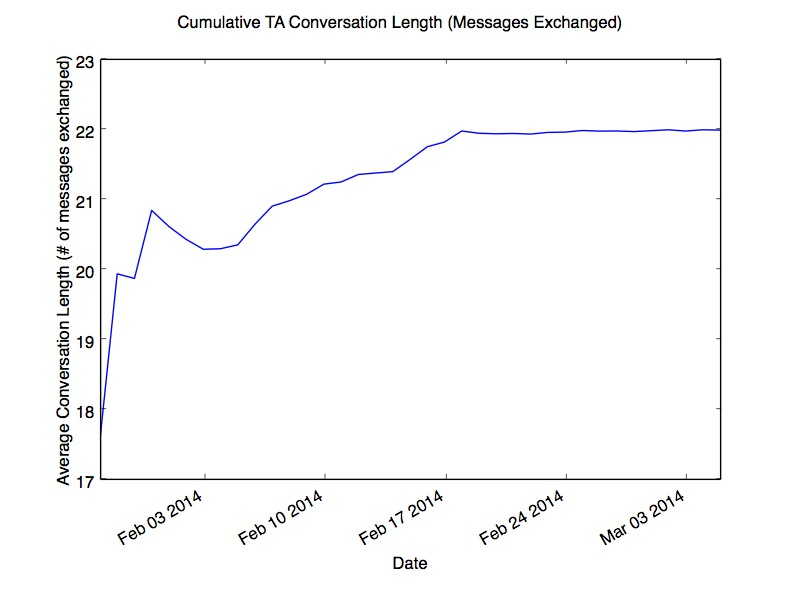
\includegraphics[trim= 0mm 0mm 0mm 0mm, clip, scale=0.5]{./Figures/CumulativeTAConversationLength(MessagesExchanged).jpg}
\caption{TA Cumulative Average Conversation Length}
\label{fig:TAMessagesExchangedCumulative}
\end{figure}

By these metrics, it seems that conversation quality improved noticeably over the course of the user experience, which suggests that the UCB1-AKSB algorithm may still have had a positive effect on conversation quality even though some of its fundamental assumptions weren't true.

\section{Individual User Analysis}
\label{sec:IndividualUserAnalysis}

Another way of examining the data is to look at how individual users as they continued to interact with the site. In each of the plots below, the x-axis represents the number of uses, while the y-axis represents the conditional mean of the metric over the set of users on the $n$-th use, given that they've used the site greater than or equal to n times. In order to define this more clearly, I introduce the following notation: let $f_k(u, n)$ give the value of conversational quality metric $k$ for user $u$ on their $n$-th visit and function $g(u)$ give the number of times user $u$ has visited the site. Let $U_n$ be the set $\{u | u \in {U}, g(u) \geq{n}\}$ (i.e. the set of users who have visited the site at least $n$ times). Then, the graphs below are plots of the following functions $y_k(n)$ for different conversational quality metrics $k$.

$$ y_k(n) = \frac{1}{|U_n|}\sum_{u \in U_n}{f_k(u, n)} $$

\begin{figure}[H]
\centering
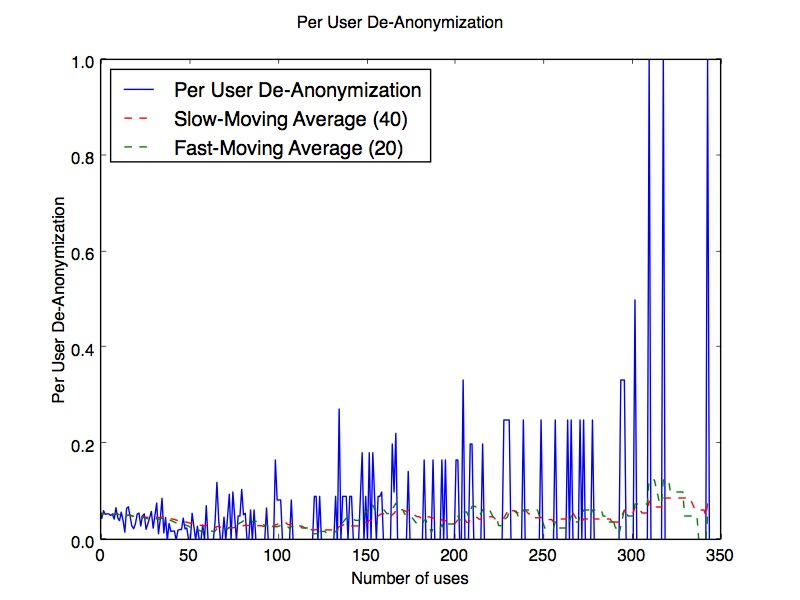
\includegraphics[trim= 0mm 0mm 0mm 0mm, clip, scale=0.5]{./Figures/PerUserDe-Anonymization.jpg}
\caption{De-Anonymization Rate Per User}
\label{fig:PerUserFBConnect}
\end{figure}

\begin{figure}[H]
\centering
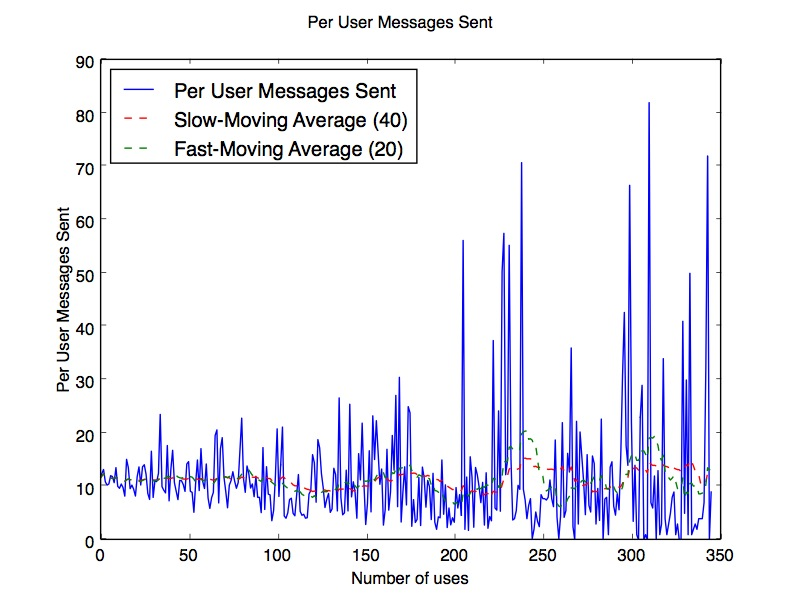
\includegraphics[trim= 0mm 0mm 0mm 0mm, clip, scale=0.5]{./Figures/PerUserMessagesSent.jpg}
\caption{Total Messages Sent Per User}
\label{fig:PerUserMessagesSent}
\end{figure}

\begin{figure}[H]
\centering
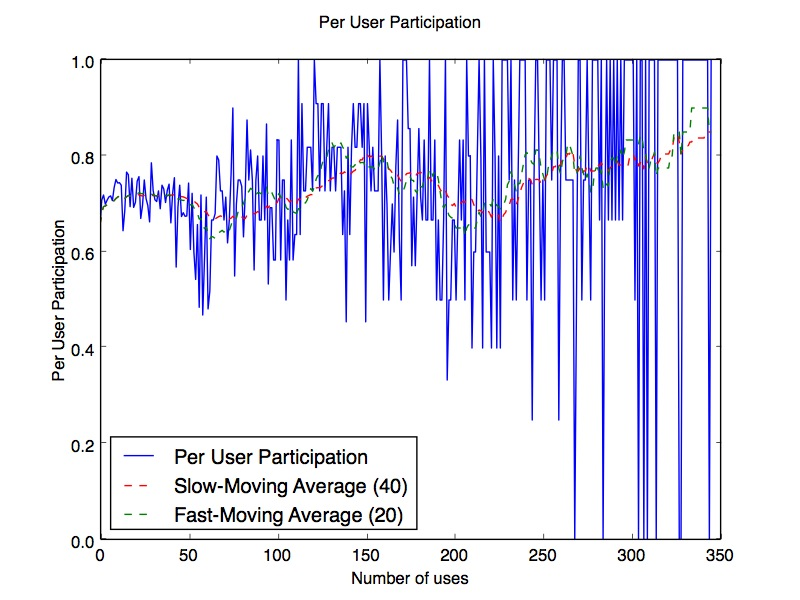
\includegraphics[trim= 0mm 0mm 0mm 0mm, clip, scale=0.5]{./Figures/PerUserParticipation.jpg}
\caption{Participation Rate Per User}
\label{fig:PerUserParticipation}
\end{figure}

The two things that immediately stand out about these plots are the general upward drift over time and increasing volatility over time. The general upward drift of each conversation quality metric on a user-level supports the hypothesis that the UCB1-AKSB was increasing conversation quality over time. Another possible source of this upward drift is that users who visit the site frequently (who I will refer to as power-users) are more interested in having high-quality conversations and will seek to do so independently of the conversation starter. However, even if the latter hypothesis is true, the UCB1-AKSB algorithm still succeeded in providing a set of initial conversation starters to these users to make them want to become power-users, so there is still evidence that the UCB1-AKSB algorithm was effective. Additionally, the steady increase in conversation de-anonymization rate (\autoref{PerUserFBConnect}) suggests that the algorithm actually performed quite well on a per-user basis, even though the cumulative de-anonymization performance was relatively poor (\autoref{TADe-AnonymizationCumulative}).

On the other hand, the increasing volatility over time of each conversation quality metric represents the stratification of users into different classes. An abrupt change from a participation rate of 1.0 to 0.0 in one use is most likely the result of a power-user being paired with an first-time user, so that the first-time user disconnects from the conversation before the power-user has a chance to participate at all.

This stratification of users into extremely high and extremely low involvement raises the issue of user saturation: people were either hooked and used the site extremely frequently or they used it a few times and then left. As a result, the site became saturated with a small fraction of hard-core users, and a large segment of users visited the site infrequently at best. This would result in poor user experience for both classes of users: the new users still have't gotten used to the idea of an anonymous conversation and might be intimidated by a conversation with a power-user, but bored with a conversation with another new-user. Conversely, a power-user would be used to the concept of an anonymous conversation and would be interested in a real conversation: they would most likely get bored with the small-talk of a new user (who still is operating in normal conversation mode) but would quickly run out of new power users to talk to. 

The solution to this problem is to have a `casual user': one who can bridge the gap between the two previous user categories and provide a better TA experience for all. However, the problem that TA ran into with Princeton is the size of the potential user base: people at Princeton who would rather use TA over socializing with their current friends. This user base is not very large, but what if it were possible to combine such a user base from multiple schools into an even larger user base? This is the motivation for the project that I'm currently working on: a larger version of Tigers Anonymous called Campus Anonymous, which will be released to all the universities in the Ivy League, thus broadening the user base and increasing the likelihood of attracting a non-trivial set of `casual users'.


\chapter{Conclusions}
\label{ch:Conclusion}
The purpose of this thesis was to test a new, weakly context-dependent multi-armed bandit algorithm that not only balances exploration and exploitation, but also prioritizes novelty to each end-user of the recommendation algorithm. This new algorithm takes advantage of data from all other users, which allows it to scale well BLAH. 

In order to test this new algorithm (UCB1-AKSB), I implemented an anonymous chatroom that I helped build and set it to optimize for maximizing conversation de-anonymizations. After collecting and analyzing conversation and user data, we can draw the following conclusions about the UCB1-AKSB algorithm. 

First, it seems that the algorithm improved some conversation quality metrics but not the metric for which it was calibrated. This is probably due to the fact that the success metric (conversation de-anonymization) was not only dependent on conversation quality (and in some cases might have been negatively correlated) and 2) a binary variable was not fine-grained enough for the size of the data-set that was available. When looking at other metrics of conversation quality, however, it does seem that the algorithm resulted in some noticeable improvement in conversation quality.

Second, the regret analysis

\section{Future Improvements}

Although the performance of the algorithm was mixed 

- Although this is disheartening, there is still room for future testing of this algorithm using other more fine-grained metrics.
- IMPROVEMENTS
	- Need more users, because problem of saturation mentioned above
	- Calibrate on more fine-grained metrics, so that algorithm decisions won't be thrown off so easily
	- Sliding window to allow for fixed set of arms to be re-cycled optimally

For a fixed arm space (i.e. Tigers Anonymous conversation starters), a possible improvement to the UCB1-AKSB algorithm would be to have a moving time-window, so that both users would be guaranteed to see a conversation starter that they haven't seen in at least 5 uses or 5 days (i.e. number of uses or a fixed time length)

FURTHER APPLICATIONS
- A weakly contextual bandit that requires less computation
- Could be used for recommendation algorithms that need to recommend newly generated content (such as blog posts, news websites, etc.) to a relatively homogenous user base


\appendix
\chapter{Data Analysis Code}
\label{app:DataAnalysisCode}
HI FIXME PLEASE


\chapter{Conversation Starters}
\label{app:ConversationStarters}
\input{./Chapters/conversation_starters}

\chapter{TA Back-End Implementation}
\label{app:TABackendImplementation}
The following pieces of code implement the back-end and front-end functionality of Tigers Anonymous unrelated to the UCB1-AKSB algorithm.

\section{Princeton IP-Address Filtering Functionality}

\begin{lstlisting}

var range_check = require('range_check');

// Pre-defined Princeton IP address blocks
var princetonIPs = [
  "128.112.0.0/16",
  "140.180.0.0/16",
  "204.153.48.0/22",
  "66.180.176.0/24",
  "66.180.177.0/24",
  "66.180.180.0/22"
];

// Check to ensure that the user's IP is a valid Princeton IP
var isValidIP = function (userIP) {
  if (userIP === "127.0.0.1" || // for debugging
      range_check.in_range(userIP, "192.168.0.0/16") ||
      range_check.in_range(userIP, "10.0.0.0/8")) {
    return true;
  }
  for (var i = 0; i < princetonIPs.length; i++) {
    if (range_check.in_range(userIP, princetonIPs[i])) {
      return true;
    }
  }
  return false;
}

exports.isValidIP = isValidIP;

\end{lstlisting}

\section{User Matching Functionality}

\begin{lstlisting}

var mongoose = require('mongoose');
var Conversation = mongoose.model('Conversation');
var ucb = require('./ucb');
var mailer = require('./mailer');

function User(socket, userID) {
  this.socket = socket;
  this.id = userID;
  this.partner = null;
  this.conversation = null;
  this.buttonClicked = false;
  this.messagesSent = 0;
  this.name = null;
  this.fbLink = null;

  var user = this;
  this.socket.on('disconnect', function() {
    if (!user.conversation) return;

    if (!user.conversation.endTime) {
      user.conversation.chatLog.push({
        date: new Date(),
        user: '',
        text: '*** ' + user.pseudonym + ' disconnected ***'
      });

      user.conversation.endTime = new Date();
      user.conversation.save();
      user.partner.socket.emit('finished');
      user.partner.socket.disconnect();
    }
  });

  this.socket.on('chat message', function(data) {
    if (!user.conversation) return;

    user.conversation.chatLog.push({
      date: new Date(),
      user: user.pseudonym,
      text: data.message
    });

    user.messagesSent++;
    user.socket.emit('chat message', {
      name: 'You',
      message: data.message
    });

    var userName = user.conversation.revealed ? user.name : 'Anonymous Tiger';
    user.partner.socket.emit('chat message', {
      name: userName,
      message: data.message
    });
  });

  this.socket.on('dropdown displayed', function(data) {
    if (!user.conversation) return;

    user.conversation.buttonDisplayed = true;
  });

  this.socket.on('identity', function(data) {
    if (!user.conversation) return;

    user.conversation.chatLog.push({
      date: new Date(),
      user: '',
      text: '*** ' + user.pseudonym + ' accepted dropdown ***'
    });

    user.name = data.name;
    user.fbLink = data.link;
    user.buttonClicked = true;

    if (user.partner.buttonClicked) {
      user.socket.emit('reveal', {
        name: user.partner.name,
        link: user.partner.fbLink
      });
      user.partner.socket.emit('reveal', {
        name: user.name,
        link: user.fbLink
      });
      user.conversation.revealed = true;

      user.conversation.chatLog.push({
        date: new Date(),
        user: '',
        text: '*** Facebook identities revealed ***'
      });
    }
  });

  this.socket.on('typing', function() {
    if (!user.conversation) return;

    user.partner.socket.emit('typing');
  });

  this.socket.on('not typing', function() {
    if (!user.conversation) return;

    user.partner.socket.emit('not typing');
  });
}

function ConversationWrapper() {
    this.user1 = null;
    this.user2 = null;
    this.startTime = new Date();
    this.endTime = null;
    this.question = null;
    this.buttonDisplayed = false;
    this.revealed = false;
    this.chatLog = [];

    var self = this;
    this.save = function() {
      new Conversation({
        userID1: self.user1.id,
        userID2: self.user2.id,
        question: self.question,
        startTime: self.startTime,
        endTime: self.endTime,
        buttonDisplayed: self.buttonDisplayed,
        user1Clicked: self.user1.buttonClicked,
        user2Clicked: self.user2.buttonClicked,
        user1MessagesSent: self.user1.messagesSent,
        user2MessagesSent: self.user2.messagesSent
      }).save();

      if (process.env.NODE_ENV === 'production') {
        mailer.sendMail(this);
      }
    };
}

var queue = new Array();
exports.connectChatter = function(socket, userID) {
  var user = new User(socket, userID);

  user.socket.emit('entrance');
  user.socket.emit('waiting');

  if (queue.length === 0) {
    queue.push(user);

    user.socket.on('disconnect', function() {
      var index = queue.indexOf(user);
      if (index !== -1) {
        queue.splice(index, 1);
      }
    });
  } else {
    var conversation = new ConversationWrapper();
    conversation.user1 = user;
    user.conversation = conversation;
    user.pseudonym = 'Origin';

    var partner = queue.shift();
    user.partner = partner;
    partner.partner = user;
    conversation.user2 = partner;
    partner.conversation = conversation;
    partner.pseudonym = 'Black';

    ucb.getQuestion(Conversation, user, partner, function(question) {
      user.conversation.question = question;
      user.socket.emit('matched', {
        question: question
      });
      partner.socket.emit('matched', {
        question: question
      });

      conversation.chatLog.push({
        date: new Date(),
        user: '',
        text: question
      });
    });
  }
};

\end{lstlisting}

\section{Web Server Functionality}

\begin{lstlisting}

var express = require('express'),
    app = express(),
    server = require('http').createServer(app),
    io = require('socket.io').listen(server);
    mongoose = require('mongoose'),
    princeton = require('./server/princeton'),
    conversation = require('./server/conversation'),
    chatter = require('./server/chatter');

var port = process.env.PORT || 5000;
server.listen(port);

var mongoUrl;
io.configure('development', function() {
  mongoUrl = 'mongodb://localhost/test';
});
io.configure('production', function() {
  mongoUrl = process.env.MONGOHQ_URL;
});
mongoose.connect(mongoUrl);

var connectedUsers = {};

app.get('/count', function(req, res) {
  var count = Object.keys(connectedUsers).length;
  res.send(count.toString());
});

io.configure('production', function() {
  io.set('log level', 1);
  io.set('transports', ['websocket']);

  io.set('authorization', function(handshakeData, callback) {
    // Check if Princeton IP
    var ipAddr = getClientIP(handshakeData);
    var isValidIP = princeton.isValidIP(ipAddr);
    if (!isValidIP) {
      callback('Sorry, this site is only for Princeton students!', false);
      return;
    }

    // Check if already connected to server
    if (ipAddr in connectedUsers) {
      callback('Sorry, you can only chat with one person at a time!', false);
      return;
    }

    callback(null, true);
  });
});

// Needed to get the client's IP on Heroku for socket.io
function getClientIP(handshakeData) {
  var forwardedIps = handshakeData.headers['x-forwarded-for'];
  if (forwardedIps) {
    return forwardedIps.split(', ')[0];
  } else {
    return handshakeData.address.address;
  }
}

function getValueFromCookie(name, cookie) {
  if (cookie) {
    var pairs = cookie.split('; ');
    for (var i = 0; i < pairs.length; i++) {
      var pair = pairs[i].split('=');
      if (pair[0] === name) {
        return pair[1];
      }
    }
  }
}

io.sockets.on('connection', function(socket) {
  var userID = getValueFromCookie('userID', socket.handshake.headers.cookie);
  if (userID) {
    // Add user to list of connected users
    var ipAddr = getClientIP(socket.handshake);
    connectedUsers[ipAddr] = true;
    socket.on('disconnect', function() {
      delete connectedUsers[ipAddr];
    });

    chatter.connectChatter(socket, userID);
  } else {
    socket.disconnect();
  }
});


\end{lstlisting}

\section{Conversation Metadata Logging Model}

\begin{lstlisting}
var mongoose = require('mongoose');

var conversationSchema = new mongoose.Schema({
  userID1: String,
  userID2: String,
  startTime: Date,
  endTime: Date,
  question: String,
  buttonDisplayed: Boolean,
  user1Clicked: Boolean,
  user2Clicked: Boolean,
  user1MessagesSent: Number,
  user2MessagesSent: Number
});

mongoose.model('Conversation', conversationSchema);
\end{lstlisting}


\chapter{TA Front-End Implementation}
\label{app:TAFrontendImplementation}
\section{Homepage}

The homepage (shown below in \ref{fig:TAHomepage}) is implemented with the code shown at the bottom of this section.

\begin{figure}[h]
\centering
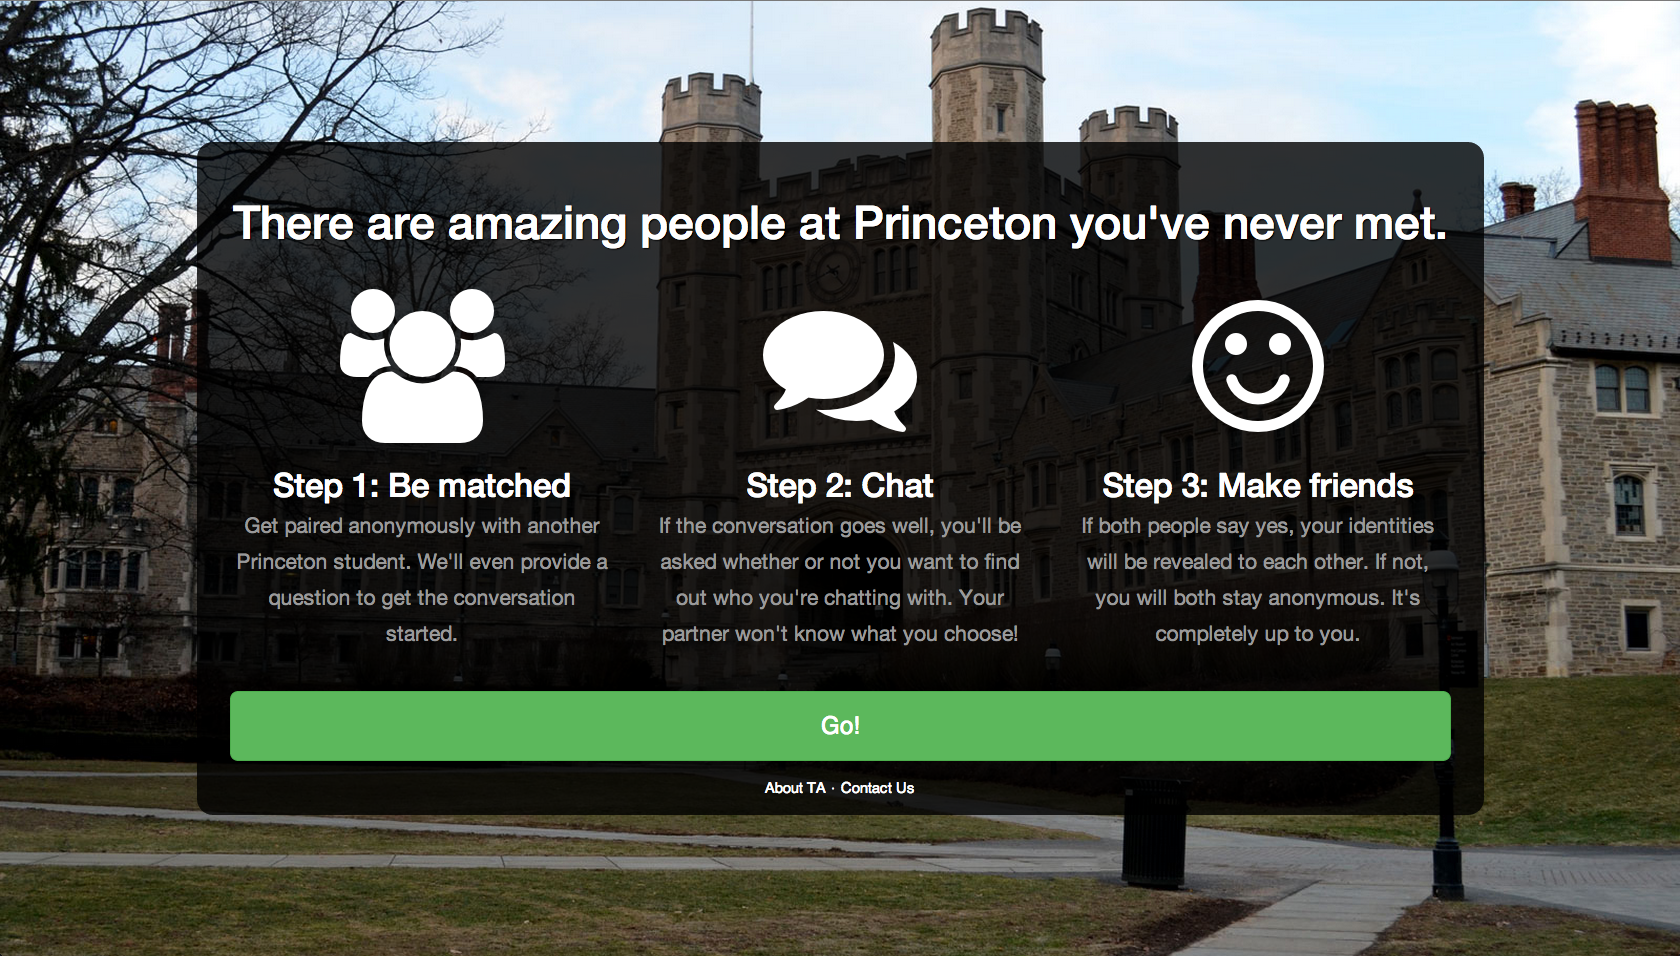
\includegraphics[trim= 35mm 0mm 35mm 0mm, clip, scale=0.25]{./Figures/TAHomepage}
\caption{Tigers Anonymous Homepage}
\label{fig:TAHomepage}
\end{figure}

\lstset{language=HTML}
\begin{lstlisting}

<!DOCTYPE html>
<html>
  <head prefix="og: http://ogp.me/ns#">
    <title>Tigers Anonymous</title>
    <link rel="icon" href="img/favicon.ico" type="image/x-icon">
    <meta name="viewport" content="width=device-width, initial-scale=1.0, user-scalable=no">
    <meta property="og:title" content="Tigers Anonymous">
    <meta property="og:description" content="There are amazing people at Princeton you've never met.">
    <meta property="og:url" content="http://www.tigersanonymous.com">
    <meta property="og:image" content="http://www.tigersanonymous.com/img/ta1024.png">
    <meta property="og:image:type" content="image/png">
    <meta property="og:image:width" content="1024">
    <meta property="og:image:height" content="1024">
    <link rel="stylesheet" href="//netdna.bootstrapcdn.com/bootstrap/3.0.3/css/bootstrap.min.css">
    <link href="//netdna.bootstrapcdn.com/font-awesome/4.0.3/css/font-awesome.css" rel="stylesheet">
    <link href="css/index.css" rel="stylesheet" type="text/css" media="all">
    <script>
      (function(i,s,o,g,r,a,m){i['GoogleAnalyticsObject']=r;i[r]=i[r]||function(){
      (i[r].q=i[r].q||[]).push(arguments)},i[r].l=1*new Date();a=s.createElement(o),
      m=s.getElementsByTagName(o)[0];a.async=1;a.src=g;m.parentNode.insertBefore(a,m)
      })(window,document,'script','//www.google-analytics.com/analytics.js','ga');
      ga('create', 'UA-23357698-2', 'tigersanonymous.com');
      ga('send', 'pageview');
    </script>
  </head>
  <body class="cover">
    <div class="wrapper">
      <div class="container">
        <div class="row text-center">
          <div class="col-md-12">
            <h1 class="hook">There are amazing people at Princeton you've never met.</h1>
          </div>
        </div>
        <div class="row how-it-works">
          <div class="col-md-4">
            <div class="row text-center padded-icon">
              <i class="fa fa-users large-icon"></i>
            </div>
            <div class="row text-center padded-text">
              <h2>
                Step 1: Be matched<br>
                <small>Get paired anonymously with another Princeton student. We'll even provide a question to get the conversation started.</small>
              </h2>
            </div>
          </div>
          <div class="col-md-4">
            <div class="row text-center padded-icon">
              <i class="fa fa-comments large-icon"></i>
            </div>
            <div class="row text-center padded-text">
              <h2>
                Step 2: Chat<br>
                <small>If the conversation goes well, you'll be asked whether or not you want to find out who you're chatting with. Your partner won't know what you choose!</small>
              </h2>
            </div>
          </div>
          <div class="col-md-4">
            <div class="row text-center padded-icon">
              <i class="fa fa-smile-o large-icon"></i>
            </div>
            <div class="row text-center padded-text">
              <h2>
                Step 3: Make friends<br>
                <small>If both people say yes, your identities will be revealed to each other. If not, you will both stay anonymous. It's completely up to you.</small>
              </h2>
            </div>
          </div>
        </div>
        <div class="row">
          <div class="col-md-12">
            <a href="/chat" class="go-btn btn btn-success btn-xlg btn-block">Go!</a>
          </div>
        </div>
        <div class="row text-center">
          <div class="col-md-12 footer">
            <a href="/about">About TA </a>
            &#8901;
            <a href="mailto:originblack609@gmail.com"> Contact Us</a>
          </div>
        </div>
      </div>
    </div>
  </body>
</html>

\end{lstlisting}

\section{About Page}

The About page (shown below in \ref{fig:TAAbout}) is implemented with the code shown at the bottom of this section.

\begin{figure}[h]
\centering
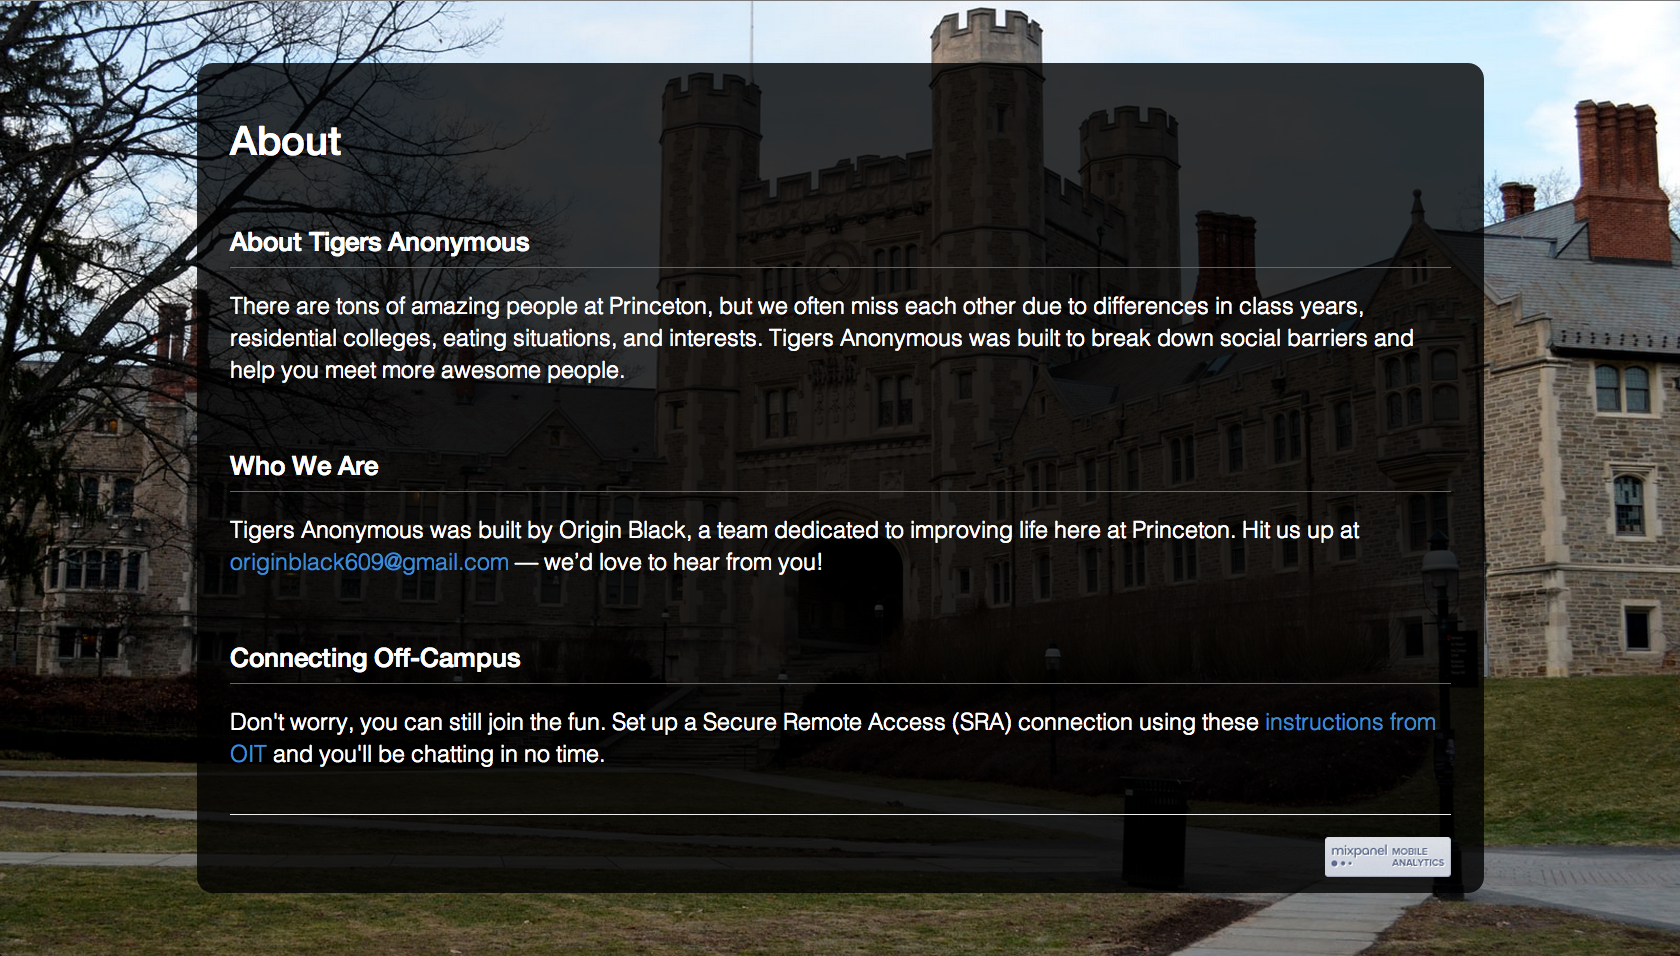
\includegraphics[trim= 35mm 0mm 35mm 0mm, clip, scale=0.25]{./Figures/TAAbout}
\caption{Tigers Anonymous About Page}
\label{fig:TAAbout}
\end{figure}

\lstset{language=HTML}
\begin{lstlisting}
<!DOCTYPE html>
<html>
  <head>
    <title>About - Tigers Anonymous</title>
    <link rel="icon" href="img/favicon.ico" type="image/x-icon">
    <meta name="viewport" content="width=device-width, initial-scale=1.0, user-scalable=no">
    <link rel="stylesheet" href="//netdna.bootstrapcdn.com/bootstrap/3.0.3/css/bootstrap.min.css">
    <link href="css/index.css" rel="stylesheet" type="text/css" media="all">
    <script>
      (function(i,s,o,g,r,a,m){i['GoogleAnalyticsObject']=r;i[r]=i[r]||function(){
      (i[r].q=i[r].q||[]).push(arguments)},i[r].l=1*new Date();a=s.createElement(o),
      m=s.getElementsByTagName(o)[0];a.async=1;a.src=g;m.parentNode.insertBefore(a,m)
      })(window,document,'script','//www.google-analytics.com/analytics.js','ga');
      ga('create', 'UA-23357698-2', 'tigersanonymous.com');
      ga('send', 'pageview');
    </script>
  </head>
  <body class="cover">
    <div class="wrapper">
      <div class="container">
        <div class="row">
          <div class="col-md-12">
            <h1>About</h1>
            <div class="header" id="about">
              <h3>About Tigers Anonymous</h3>
            </div>
            <p class="lead">
            There are tons of amazing people at Princeton, but we often miss each other due to differences in class years, residential colleges, eating situations, and interests. Tigers Anonymous was built to break down social barriers and help you meet more awesome people.
            </p>
            <div class="header" id="whoweare">
              <h3>Who We Are</h3>
            </div>
            <p class="lead">
            Tigers Anonymous was built by Origin Black, a team dedicated to improving life here at Princeton. Hit us up at <a href="mailto:originblack609@gmail.com">originblack609@gmail.com</a> &#8212 we�d love to hear from you!
            </p>
            <div class="header" id="offcampus">
              <h3>Connecting Off-Campus</h3>
            </div>
            <p class="lead">
            Don't worry, you can still join the fun. Set up a Secure Remote Access (SRA) connection using these <a href="http://helpdesk.princeton.edu/kb/display.plx?ID=6023">instructions from OIT</a> and you'll be chatting in no time.
            </p>
          </div>
        </div>
        <div class="row">
          <div class="col-md-12 text-right">
            <hr>
            <a href="https://mixpanel.com/f/partner"><img src="//cdn.mxpnl.com/site_media/images/partner/badge_light.png" alt="Mobile Analytics" /></a>
          </div>
        </div>
      </div>
    </div>
  </body>
</html>

\end{lstlisting}

\section{Chatroom}

The Tigers Anonymous chatroom (shown below in \ref{fig:TAChatRoom}) is implemented with the code shown at the bottom of this section.

\begin{figure}[h]
\centering
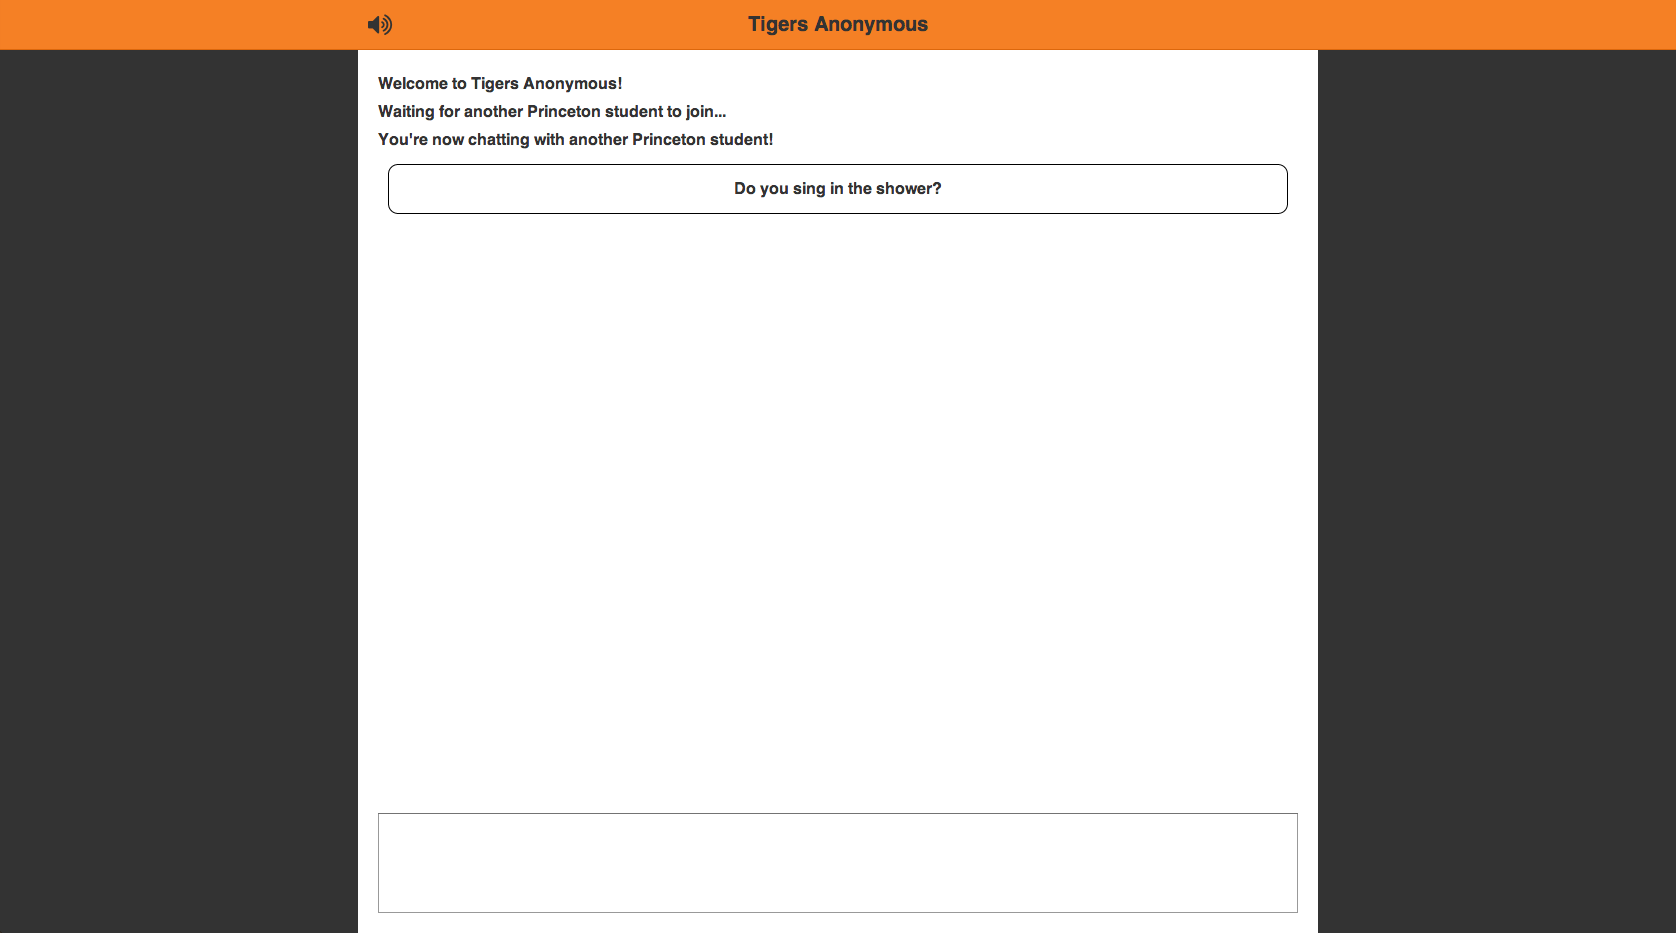
\includegraphics[trim= 35mm 0mm 35mm 0mm, clip, scale=0.25]{./Figures/TAChatroom}
\caption{Tigers Anonymous Chatroom}
\label{fig:TAChatRoom}
\end{figure}

\lstset{language=HTML}
\begin{lstlisting}

<!DOCTYPE html>
<html ng-app="pom">
  <head ng-controller="TitleCtrl">
    <title ng-bind="getTitle()">Tigers Anonymous</title>
    <link rel="icon" href="img/favicon.ico" type="image/x-icon">
    <meta name="viewport" content="width=device-width, initial-scale=1.0, user-scalable=no">
    <meta name="apple-mobile-web-app-capable" content="yes">
    <link href="//netdna.bootstrapcdn.com/font-awesome/4.0.3/css/font-awesome.css" rel="stylesheet">
    <link href="css/chat.css" rel="stylesheet" type="text/css" media="all">
  </head>
  <body ng-controller="ChatCtrl">
    <div id="fb-root"></div>
    <div class="nav">
      <div class="nav-container">
        <span class="brand" href="/">Tigers Anonymous</span>
        <a class="volume" ng-click="playSound = !playSound" ng-cloak>
          <i class="fa fa-volume-up" ng-show="playSound"></i>
          <i class="fa fa-volume-off" ng-show="!playSound"></i>
        </a>
        <a class="circle-down" ng-show="dropdown.shouldShowMinimized() && state == 'chatting'" ng-click="dropdown.show()" ng-cloak>
          <i class="fa fa-chevron-circle-down"></i>
        </a>
      </div>
    </div>
    <div class="chat-container">
      <div class="dropdown" ng-show="dropdown.shouldShowFull() && state == 'chatting'" ng-cloak>
        <div class="question">
          Do you want to find out who you've been chatting with?<br>
          <span class="promise">We'll never post to Facebook without your permission. Promise.</span>
        </div>
        <div class="options">
          <button type="button" class="yes-btn" ng-click="dropdown.accept()">Yes</button>
          <button type="button" class="hide-btn" ng-click="dropdown.hide()">Hide</button>
        </div>
      </div>
      <div class="chatroom" pom-scroll-glue>
        <ul ng-cloak>
          <li ng-repeat="message in messages" ng-class="message.type" ng-switch="message.type">
            <div ng-switch-when="chat">
              <span ng-class="{userName: !message.isPartner, partnerName: message.isPartner}">{{message.name}}:</span>
              <span ng-bind-html="message.text | linky | linkyNewlines"></span>
            </div>
            <div ng-switch-when="system">
              <div ng-switch="message.template" ng-class="{important: message.important}">
                <div ng-switch-when="entrance">
                  Welcome to Tigers Anonymous!
                </div>
                <div ng-switch-when="waiting">
                  Waiting for another Princeton student to join...
                </div>
                <div ng-switch-when="matched">
                  You're now chatting with another Princeton student!<br>
                  <div class="question-box">
                    {{message.question}}
                  </div>
                </div>
                <div ng-switch-when="selfRevealed">
                  Your partner's identity will be revealed if they also want to discover yours.
                </div>
                <div ng-switch-when="partnerRevealed">
                  Congratulations! You get to find out your partner's identity!<br>
                  You've been chatting with: <a href="{{message.partnerLink}}" target="_blank">{{message.partnerName}}</a>
                </div>
                <div ng-switch-when="fbError">
                  Sorry, there was an error connecting to Facebook. Please try again.
                </div>
                <div ng-switch-when="fbFake">
                  Sorry, it looks like you're using a fake Facebook account.
                </div>
                <div ng-switch-when="finished">
                  {{partnerName}} has disconnected. Refresh the page to start another chat!<br>
                  What do you think about Tigers Anonymous? <a href="https://docs.google.com/forms/d/1NI2nuAoYRZzYcawLrbWPKHsc43EdvbS5mU5d0A4cM2U/viewform" target="_blank">Let us know!</a>
                </div>
                <div ng-switch-when="disconnected">
                  You have been disconnected.
                </div>
                <div ng-switch-when="error">
                  Sorry, we're unable to connect you. Please check the following:
                  <ol>
                    <li>
                    You need to be using a computer connected to Princeton's network.<br>
                    If you're off-campus, <a href="about#offcampus">follow these instructions.</a>
                    </li>
                    <li>You can't already be chatting with a user.</li>
                    <li>You need to be using a modern web browser that supports WebSockets.</li>
                  </ol>
                </div>
                <div ng-switch-default>
                  {{message.text}}
                </div>
              </div>
            </div>
          </li>
          <li class="typing" ng-show="partnerTyping && state == 'chatting'">
            {{partnerName}} is typing...
        </ul>
      </div>
      <div class="input-wrapper">
        <textarea
          tabindex="1"
          pom-focus-on-chat
          ng-disabled="state != 'chatting'"
          ng-model="message"
          ng-keydown="sendMessage($event)"
          ng-change="updateTyping()"></textarea>
      </div>
    </div>
    <audio pom-play-on-message src="audio/notification.wav"></audio>
    <script src="/socket.io.js"></script>
    <script src="//ajax.googleapis.com/ajax/libs/angularjs/1.2.6/angular.min.js"></script>
    <script src="//ajax.googleapis.com/ajax/libs/angularjs/1.2.6/angular-sanitize.js"></script>
    <script src="//ajax.googleapis.com/ajax/libs/angularjs/1.2.6/angular-animate.js"></script>
    <!-- build:js js/app.js -->
    <script src="js/app.js"></script>
    <script src="js/controllers.js"></script>
    <script src="js/directives.js"></script>
    <script src="js/services.js"></script>
    <script src="js/filters.js"></script>
    <!-- endbuild -->
  </body>
</html>

\end{lstlisting}


\bibliographystyle{plainnat}
\bibliography{./Bibliography/refs}
\end{document}
